\documentclass{standalone}
\usepackage{tikz}

\begin{document}

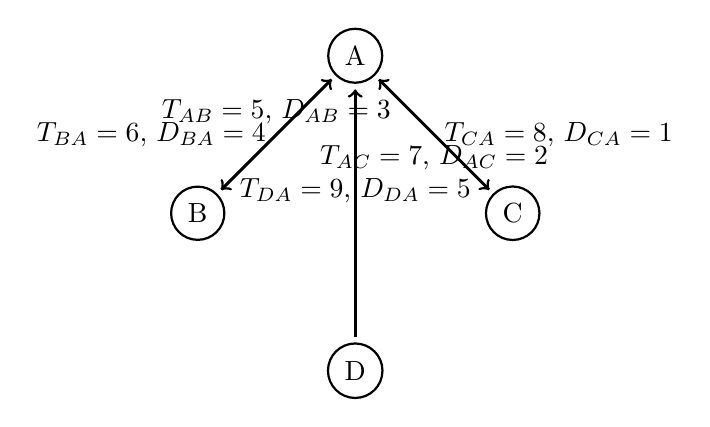
\begin{tikzpicture}[node distance=2cm, thick]

    % Define styles for nodes and edges
    \tikzset{
        nodeStyle/.style={circle, draw, fill=white, minimum size=10pt},
        edgeStyle/.style={->, bend left, shorten >=2pt, shorten <=2pt, line width=1pt}
    }

    % Nodes
    \node[nodeStyle] (A) at (0,0) {A};
    \node[nodeStyle] (B) at (-2,-2) {B};
    \node[nodeStyle] (C) at (2,-2) {C};
    \node[nodeStyle] (D) at (0,-4) {D};

    % Edges with labels
    \draw[edgeStyle] (A) -- node[above] {$T_{AB} = 5$, $D_{AB} = 3$} (B);
    \draw[edgeStyle] (A) -- node[below] {$T_{AC} = 7$, $D_{AC} = 2$} (C);
    \draw[edgeStyle] (B) -- node[left] {$T_{BA} = 6$, $D_{BA} = 4$} (A);
    \draw[edgeStyle] (C) -- node[right] {$T_{CA} = 8$, $D_{CA} = 1$} (A);
    \draw[edgeStyle] (D) -- node[above] {$T_{DA} = 9$, $D_{DA} = 5$} (A);

\end{tikzpicture}

\end{document}